\section{Warmup Convergence}\label{warmup-convergence}

At the beginning of each new environment (design day or runperiod) zone and surface temperatures are initialized to 23C, and zone humidity ratios are initialized to the outdoor humidity ratio. The first day of the environment is repeated until the loads/temperature convergence tolerance values specified in the Building object are satisfied or until it reaches ``maximum number of warmup days''.

Since everything in EnergyPlus is based on the foundation of the loads simulation, it stands to reason that any inaccuracies in the loads calculation will result in inaccuracies of similar or larger magnitude in the HVAC calculations. In the presumably limited cases where convergence was not truly achieved before the actual simulation began, it is unknown how much error would be introduced into the results. While simulations that last longer (annual vs.~design day) will hopefully have any initial condition problems balanced by the shear number of days in the simulation, shorter simulations---particularly those used for sizing---could result in relatively large errors. The simulation results could be unreliable and inaccurate when steady periodic conditions are not achieved. Therefore, it is important to properly determine when there is enough temperature and flux history terms to start an EnergyPlus simulation since this has a potential economic and energy impact on buildings that use EnergyPlus in design.

EnergyPlus determines warmup convergence in the following manner as shown in the Figure~\ref{fig:flows-of-warmup-convergence-checks} below. The process of the convergence checks begins by tracking four parameters such including the maximum zone air temperature, the minimum zone air temperature, the maximum heating load, and the maximum cooling load for individual zone. It is note that these convergence checks are only in effective in simulations with at least one zone since the criteria is solely based on the maximum and minimum values obtained from an individual zone. Differences in these parameters between two consecutive days are then compared with the convergence tolerance values at the end of the day during the warmup period. For example, the maximum and minimum air temperature and the percentage difference of zone load for each zone at 9:00AM during the second to last warmup is compared to the values at 9:00AM last warmup day as follows:

\begin{equation}
{T_{\max ,prev}} - {T_{\max }} < {T_{tol}}
\end{equation}

\begin{equation}
{T_{\min ,prev}} - {T_{\min }} < {T_{tol}}
\end{equation}

\begin{equation}
\frac{{{q_h} - {q_{h,prev}}}}{{{q_h}}} < {q_{tol}}
\end{equation}

\begin{equation}
\frac{{{q_c} - {q_{c,prev}}}}{{{q_c}}} < {q_{tol}}
\end{equation}

where Tmax,prev is the maximum zone temperature of previous day, Tmax is the maximum zone temperature of current day, Ttol is the value of temperature tolerance, qh,prev is the maximum heating load of previous day, qh, is the maximum heating load of current day, qtol is the value of load tolerance, qc,prev is the maximum cooling load of previous day, and qc, is the maximum cooling load of current day.

Note that a minimum load of 100W is used to establish a fraction for the maximum loads when they are less than the minimum. This is done to avoid a false negative indication for the percentage load difference that may appear when zonal loads are very small. The convergence checks are repeated until passed for all zones. EnergyPlus assumes that the warmup period has been reached steady-periodic when these four parameters are within tolerance. Finally, temperature and load differences between the last two warmup days for individual zone at each time step in the last warmup day are reported so that users can easily track whether or not the warmup period has converged. The input parameters and output related to the warmup period are discussed in the Input-Output Reference.

\begin{figure}[hbtp] % fig 2
\centering
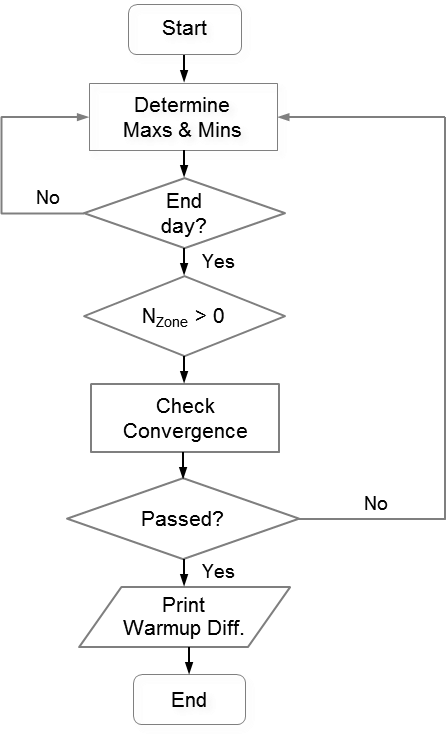
\includegraphics[width=0.9\textwidth, height=0.9\textheight, keepaspectratio=true]{media/image6.png}
\caption{Flows of Warmup Convergence Checks \protect \label{fig:flows-of-warmup-convergence-checks}}
\end{figure}
